\documentclass[USEnglish,ignorenonframetext,notheorems,aspectratio=1610]{beamer}
\usetheme[compress]{Madrid}
\usecolortheme{albatross}
\usepackage{tikz,tikzscale}
\usetikzlibrary{snakes}
\tikzset{velox/.style={color=black,draw,fill=red,thick,%
    shape=diamond,aspect=.4,
    inner sep=1.3pt,transform shape}}
\tikzset{veloy/.style={color=black,draw,fill=red,thick,%
    shape=diamond,aspect=2.5,
    inner sep=1.3pt,transform shape}}
\tikzset{veloxy/.style={color=black,draw,fill=red,thick,%
    shape=star,star points=4,star point ratio=2.2,
    inner sep=1.3pt,transform shape}}
\tikzset{pressure/.style={color=black,draw,fill=cyan,thick,%
    shape=circle,inner sep=2pt,transform shape}}
\tikzset{velo/.style={transform shape,double=red,arrows={-Stealth[open,fill=red]}}}

%% Macros for drawing degrees of freedom for different shapes/elements.
%% Arguments are always:
%%   #1: Starting point
%%   #2: End point
%%   #3: polynomial degree
%%   #4: node settings

\tikzset{pics/edgenormal/.style args={#1/#2/#3/#4}{%
    code={%
      \draw #1 -- #2
      node foreach \x [evaluate=\x as \xval] in {1,...,#3} [#4,sloped,pos=\xval/(#3+1)] {};
      }
}}


%% Macros for drawing degrees of freedom for different shapes/elements.
%% Arguments are always:
%%   #1: polynomial degree
%%   #2: node settings

\tikzset{pics/tripile/.style args={#1/#2}{%
    code={%
      \coordinate (top) at (0,#1);
      \foreach \i in{0,...,#1}
      \foreach \j in{0,...,\i}
      {
        \tikzmath{
          \y = .3*(2/3*#1-\i)*cos(30);
          \x = .3*(\i/2-\j);
        }
        \node[#2] at (\x,\y) {};
      }
    }
}}

\tikzset{pics/tensor/.style args={#1/#2/#3}{%
    code={%
      \coordinate (top) at (0,#1);
      \foreach \i in{0,...,#1}
      \foreach \j in{0,...,#2}
      {
        \tikzmath{
          \y = 2*(\i+1)/(#1+2);
          \x = 2*(\j+1)/(#2+2);
        }
        \node[#3] at (\x,\y) {};
      }
    }
}}

\tikzset{pics/pfem/.style args={#1/#2}{%
    code={%
      \tikzmath{ \ytop=2*cos(30); }
      \coordinate (top) at (0,\ytop);

      \foreach \i in{0,...,#1}
      \foreach \j in{0,...,\i}
      {
        \tikzmath{
          \y = \ytop-\ytop*\i/#1;
          \x = 2*(\i/2-\j)/#1+1;
        }
        \node[#2] at (\x,\y) {};
      }
    }
}}

\tikzset{pics/qfem/.style args={#1/#2}{%
    code={%
      \foreach \i in{0,...,#1}
      \foreach \j in{0,...,#1}
      {
        \tikzmath{
          \y = 2-2*\i/#1;
          \x = 2-2*\j/#1;
        }
        \node[#2] at (\x,\y) {};
      }
    }
}}

%%% Local Variables:
%%% mode: latex
%%% TeX-master: "all"
%%% End:

\def\restrict{r}
\def\prolongate{p}

\usepackage{../mathsim}
\usepackage{times}
\usepackage{xr}
\externaldocument{main}
\usepackage{mfirstuc}
\usepackage{mathtools}  
\mathtoolsset{showonlyrefs}

\def\footnote#1{}
\def\putindex#1{#1}
\title{Finite Elements}
\author{Guido Kanschat}
\date{\today}
\begin{document}
\frame{\maketitle}
\frame{\frametitle{Overview}\tableofcontents[hideallsubsections]}
\section{Elliptic PDE and Their Weak Formulation}
\frame{\sectoc}
\subsection{Elliptic boundary value problems}

\frame {\input{blocks/Notation-coordinates.tex}}
\frame {\input{blocks/Notation-partial-derivative.tex}}
\frame {\input{blocks/Notation-elim-coord.tex}
  \input{blocks/Definition-lin-pde-2order.tex}}
\frame {\input{blocks/Definition-poisson-eqn.tex}}
\frame {\input{blocks/Definition-domain.tex}}
\frame {\input{blocks/Definition-boundary-conditions.tex}}
\frame {\input{blocks/Definition-dirichlet-problem-differential.tex}}
\frame {\input{blocks/Theorem-Dirichlet-principle.tex}}
\frame {\input{blocks/Theorem-Dirichlet-variational-principle.tex}
  \input{blocks/Corollary-Dirichlet-uniqueness.tex}}
\frame {\input{blocks/Lemma-reduction-to-zero-bc.tex}}
\frame {\input{blocks/Notation-l2.tex}}
\frame {\input{blocks/Lemma-Friedrichs-continuous.tex}
  \input{blocks/Problem-Friedrichs.tex}}
\frame {\input{blocks/Lemma-h1-norm.tex}}
\frame {\input{blocks/Lemma-Dirichlet-energy-boundedness.tex}
  \input{blocks/Lemma-minimizing-sequence.tex}}
\frame {\input{blocks/Definition-h10.tex}
  \input{blocks/Lemma-Friedrichs-h1.tex}}
\frame {\input{blocks/Definition-weak-formulation.tex}
  \input{blocks/Theorem-weak-unique-solution-1.tex}}

\frame {\input{blocks/Lemma-neumann-weak.tex}}
\frame {\input{blocks/Definition-natural-bc.tex}}
\frame {\input{blocks/Lemma-mixed-bc-weak.tex}}

\subsection{Hilbert Spaces and Bilinear Forms}
\frame{\tableofcontents[currentsection,subsectionstyle=show/shaded/hide]}

\frame {\input{blocks/Definition-inner-product.tex}}
\frame {\input{blocks/Theorem-bcs-inequality.tex}
  \input{blocks/Lemma-inner-product-norm.tex}}
\frame {\input{blocks/Definition-complete.tex}}
\frame {\input{blocks/Definition-Banach-hilbert.tex}}
\frame {\input{blocks/Definition-orthogonal.tex}}
\frame {\input{blocks/Definition-orthogonal-complement.tex}}
\frame {\input{blocks/Lemma-orthogonal-closed.tex}}
\frame {\input{blocks/Theorem-orthogonal-complement.tex}}
% \frame {\input{blocks/Corollary-ortho-density.tex}}
\frame {\input{blocks/Definition-ortho-projection.tex}}
\frame {\input{blocks/Definition-dual-space.tex}}
\frame {\input{blocks/Theorem-Riesz-representation.tex}}
\frame {\input{blocks/Definition-bilinear-form.tex}}
\frame {\input{blocks/Lemma-pde-bilinear.tex}}
\frame {\input{blocks/Lemma-lax-milgram.tex}}
\frame {\input{blocks/Lemma-weak-well-posed.tex}
  \input{blocks/Definition-elliptic.tex}}

\subsection{Fast facts on Sobolev spaces}
\frame{\tableofcontents[currentsection,subsectionstyle=show/shaded/hide]}

\frame {\input{blocks/Notation-multi-index.tex}}
\frame {\input{blocks/Definition-distributional-derivative.tex}}
\frame {\input{blocks/Definition-Wkp.tex}
  \input{blocks/Corollary-wkp-embedding.tex}}
\frame {\input{blocks/Definition-hkp.tex}
  \input{blocks/Theorem-meyers-serrin.tex}}

\frame {\input{blocks/Definition-boundary-smoothness.tex}}
\frame {\input{blocks/Definition-continuous-embedding.tex}}
\frame {\input{blocks/Theorem-sobolev-embedding.tex}}
\frame {\input{blocks/Lemma-trace-continuous.tex}
  \input{blocks/Theorem-trace.tex}}
\frame {\input{blocks/Definition-hoelder-spaces.tex}}
\frame {\input{blocks/Theorem-hoelder-embedding.tex}
  \input{blocks/Corollary-sobolev-continuous.tex}}

\subsection{Properties of solutions}
\frame{\tableofcontents[currentsection,subsectionstyle=show/shaded/hide]}

\frame {\input{blocks/Definition-wkp-loc.tex}
  \input{blocks/Theorem-gt-8-8.tex}
  \input{blocks/Theorem-gt-8-10.tex}
  \input{blocks/Corollary-gt-8-10.tex}}
\frame {\input{blocks/Theorem-gt-8-13.tex}
  \input{blocks/Corollary-h2-solution-bvp.tex}
  \input{blocks/Remark-classical-smooth.tex}
  \input{blocks/Remark-classical-convex.tex}}
\frame {\input{blocks/Theorem-kondratev.tex}}

%%%%%%%%%%%%%%%%%%%%%%%%%%%%%%%%%%%%%%%%%%%%%%%%%%%%%%%%%%%%%%%%%%%%%%
%%%%%%%%%%%%%%%%%%%%%%%%%%%%%%%%%%%%%%%%%%%%%%%%%%%%%%%%%%%%%%%%%%%%%%
\section{Conforming Finite Element Methods}
\frame{\sectoc}
\subsection{Meshes, shape functions, and degrees of freedom}
%%%%%%%%%%%%%%%%%%%%%%%%%%%%%%%%%%%%%%%%%%%%%%%%%%%%%%%%%%%%%%%%%%%%%%
%%%%%%%%%%%%%%%%%%%%%%%%%%%%%%%%%%%%%%%%%%%%%%%%%%%%%%%%%%%%%%%%%%%%%%
\frame {\input{blocks/Definition-facets.tex}
  \input{blocks/Definition-mesh.tex}}
\frame {\input{blocks/Definition-finite-element.tex}
\input{blocks/Notation-dofs.tex}}
\frame {\input{blocks/Definition-node-topology.tex}
  \input{blocks/Definition-fe-space.tex}}
\frame {\input{blocks/Notation-global-local.tex}}
\frame {\input{blocks/Definition-local-global.tex}}
\frame {\input{blocks/Lemma-fe-support.tex}}
\frame {\input{blocks/Lemma-mesh-continuity.tex}
  \input{blocks/Lemma-nodal-continuity.tex}}

\frame {\input{blocks/Definition-barycentric-coordinates.tex}}
\frame {\input{blocks/Lemma-barycentric-affine.tex}
  \input{blocks/Corollary-barycentric-interpolation.tex}}

\begin{frame}
  \frametitle{The $P_1$ element in barycentric coordinates}
  \begin{columns}
    \begin{column}{.5\textwidth}
      \begin{center}
        \includegraphics[width=.6\textwidth]{mixed/fig/p1-p.tikz}
      \end{center}
    \end{column}
    \begin{column}{.5\textwidth}
      \begin{gather*}
        \phi_i = \lambda_i,
        \quad i=0,1,2
      \end{gather*}
    \end{column}
  \end{columns}
\end{frame}

\begin{frame}
  \frametitle{The $P_2$ element in barycentric coordinates}
  \begin{columns}
    \begin{column}{.5\textwidth}
      \begin{center}
        \includegraphics[width=.6\textwidth]{mixed/fig/p2-p.tikz}
      \end{center}
    \end{column}
    \begin{column}{.5\textwidth}
      \begin{xalignat*}2
        \phi_{ii} &= 2\lambda_i^2 - \lambda_i,
        &i&=0,1,2\\
        \phi_{ij} &= 4\lambda_i\lambda_j
        &j&\neq i
      \end{xalignat*}
    \end{column}
  \end{columns}
\end{frame}

\begin{frame}
  \frametitle{The $P_3$ element in barycentric coordinates}
  \begin{columns}
    \begin{column}{.5\textwidth}
      \begin{center}
        \includegraphics[width=.6\textwidth]{mixed/fig/p3-p.tikz}
      \end{center}
    \end{column}
    \begin{column}{.5\textwidth}
      \begin{xalignat*}2
        \phi_{iii} &= \tfrac12 \lambda_i(3\lambda_i-1)(3\lambda_i-2)
        &i&=0,1,2\\
        \phi_{ij} &= \tfrac92\lambda_i\lambda_j(3\lambda_j-1)
        &j&\neq i\\
        \phi_0 &= 27\lambda_0\lambda_1\lambda_2
      \end{xalignat*}
    \end{column}
  \end{columns}
\end{frame}

\frame {\input{blocks/Definition-galerkin-approximation.tex}}
\frame {\input{blocks/Corollary-galerkin-equations.tex}}
\frame {\input{blocks/Lemma-discrete-lax-milgram.tex}
  \input{blocks/Lemma-cea.tex}}
\frame {\input{blocks/Lemma-fe-matrix.tex}}
\frame {\input{blocks/Algorithm-matrix-assembling.tex}}

\frame {\input{blocks/Definition-tensor-product-polynomials.tex}}
\frame {\input{blocks/Lemma-tensor-product-node-functionals.tex}}

\begin{frame}
  \frametitle{Example: $Q_2$ shape functions}
  \begin{center}
    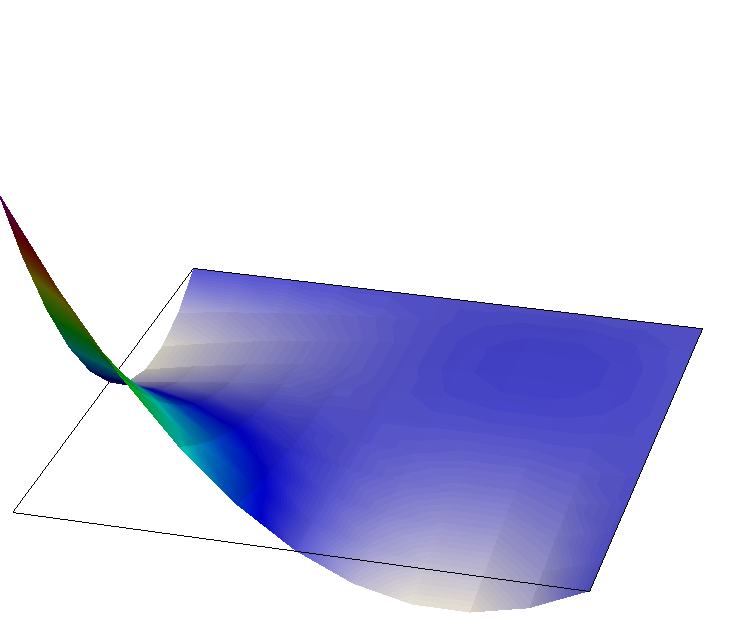
\includegraphics[height=.27\textheight]{graph/shape0}
    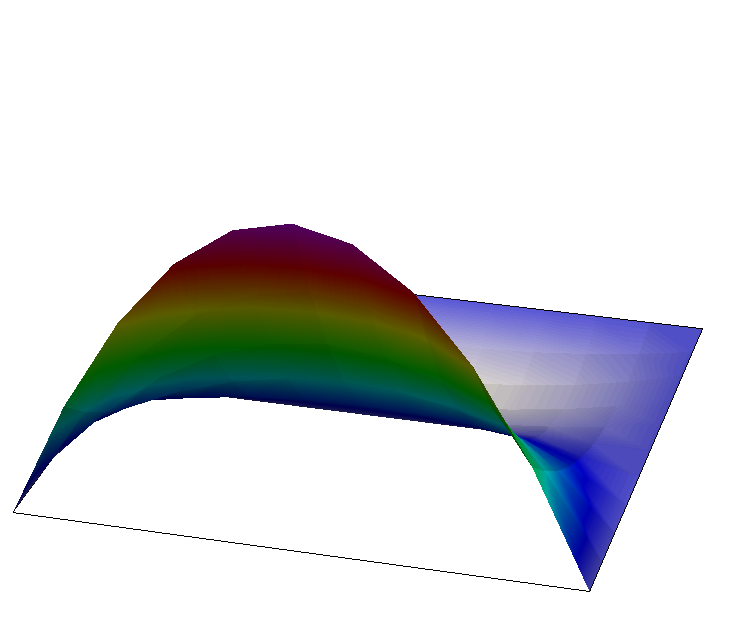
\includegraphics[height=.27\textheight]{graph/shape1}
    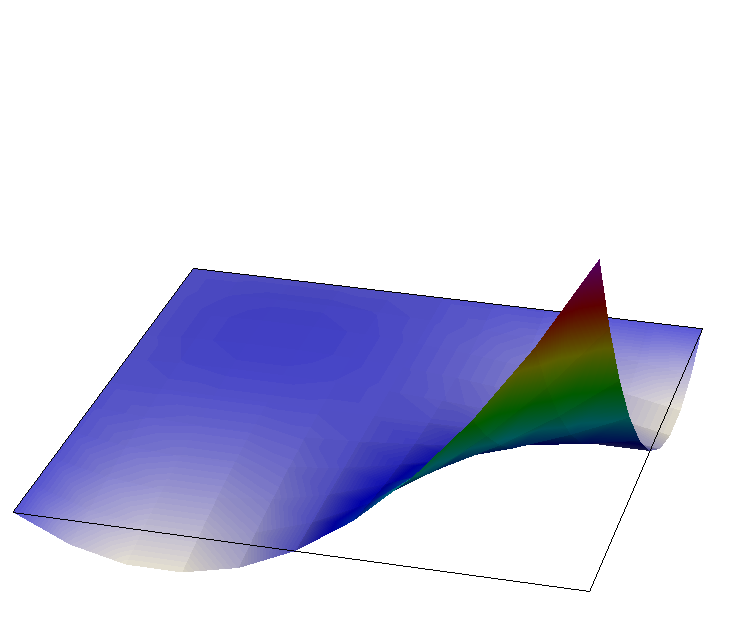
\includegraphics[height=.27\textheight]{graph/shape2}

    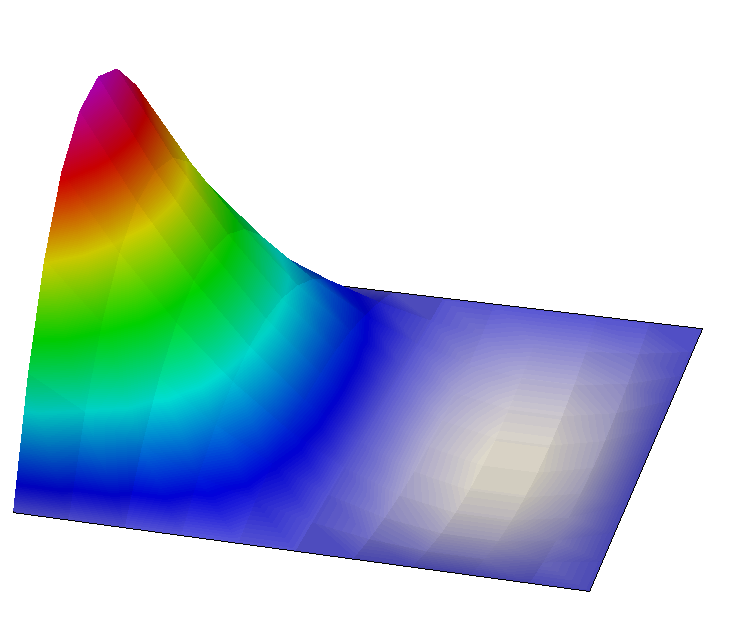
\includegraphics[height=.27\textheight]{graph/shape3}
    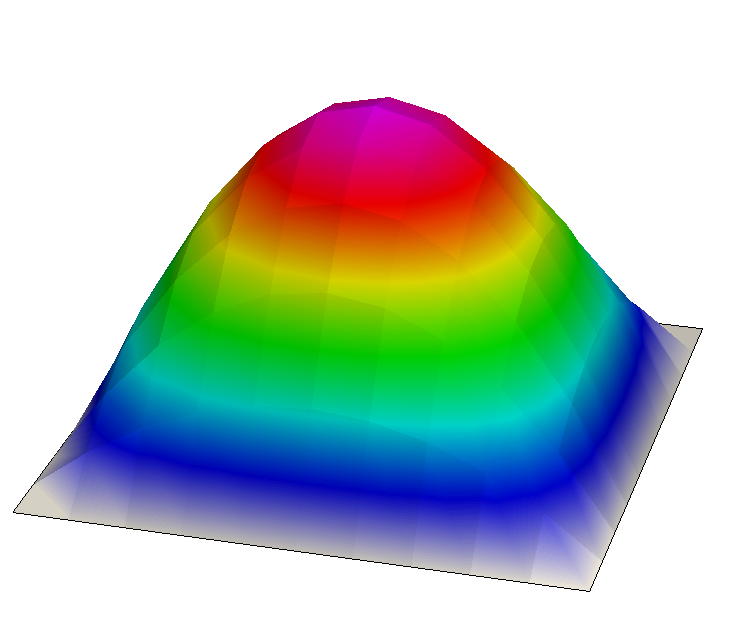
\includegraphics[height=.27\textheight]{graph/shape4}
    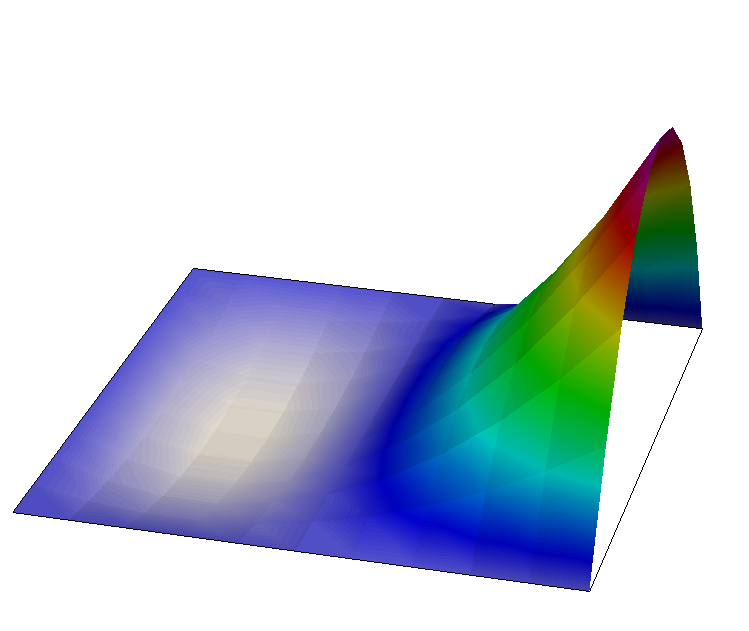
\includegraphics[height=.27\textheight]{graph/shape5}

    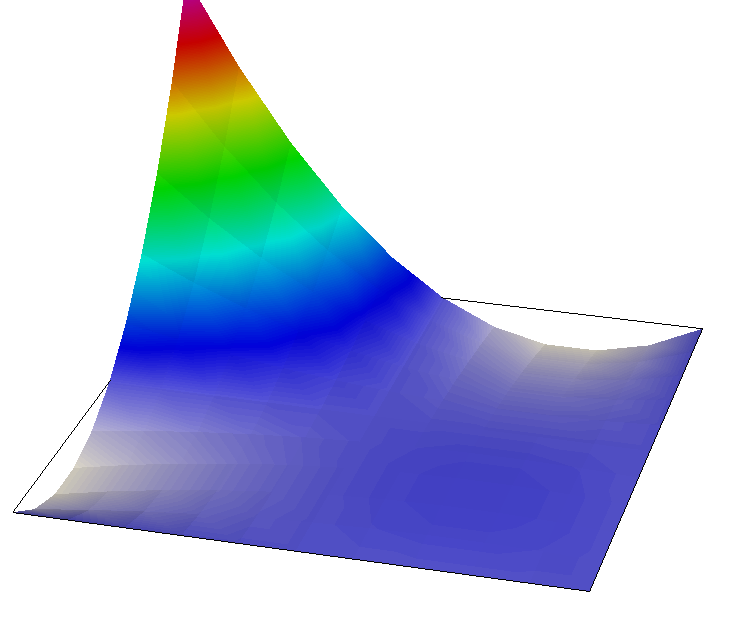
\includegraphics[height=.27\textheight]{graph/shape6}
    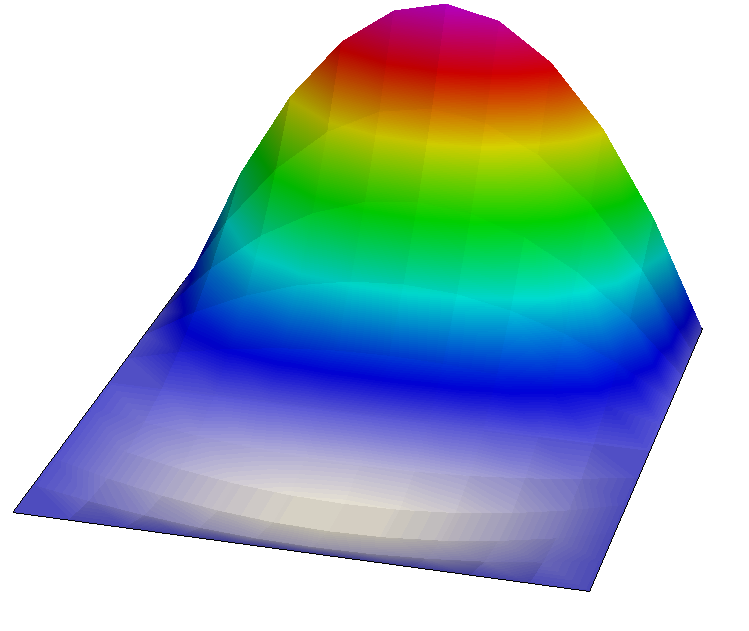
\includegraphics[height=.27\textheight]{graph/shape7}
    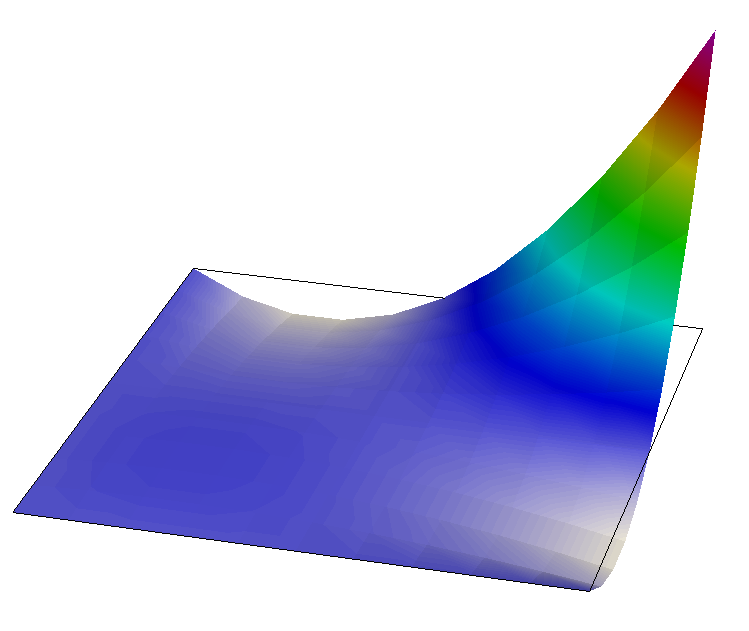
\includegraphics[height=.27\textheight]{graph/shape8}
  \end{center}
\end{frame}

\frame {\input{blocks/Lemma-tensor-product-trace.tex}}

\begin{frame}
  \frametitle{Example: $Q_2$ continuous basis (selection)}
  \begin{center}
    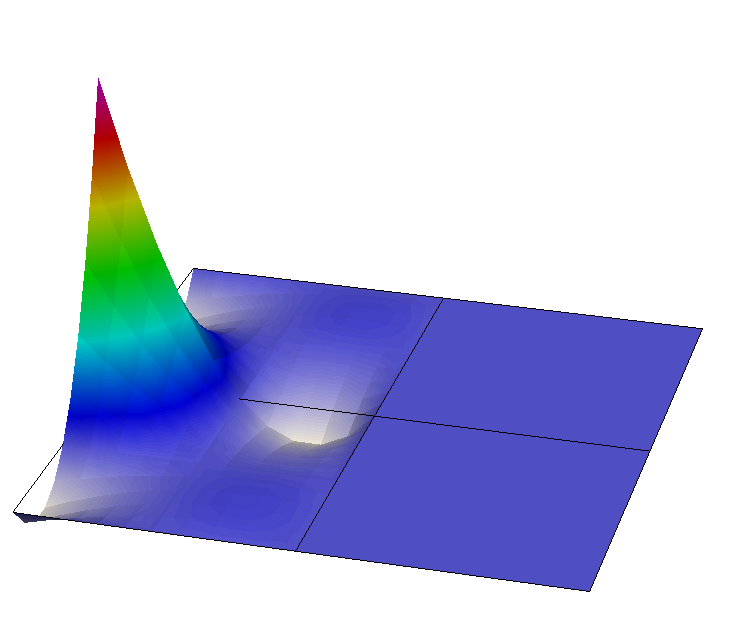
\includegraphics[height=.27\textheight]{graph/cgbasis1-02}
    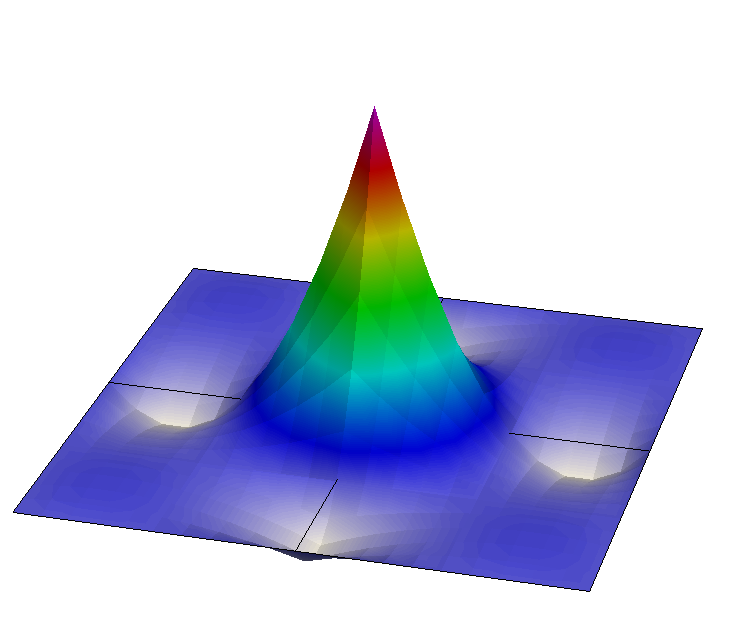
\includegraphics[height=.27\textheight]{graph/cgbasis1-03}
    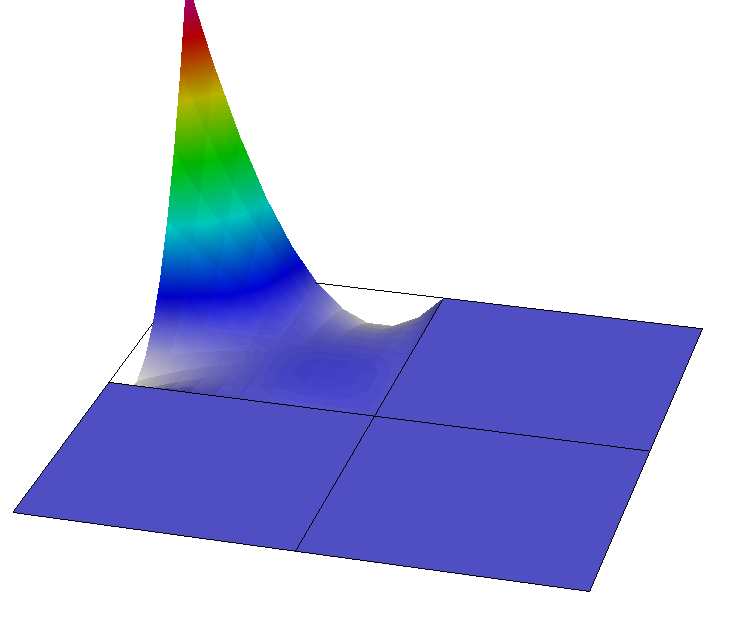
\includegraphics[height=.27\textheight]{graph/cgbasis1-15}
    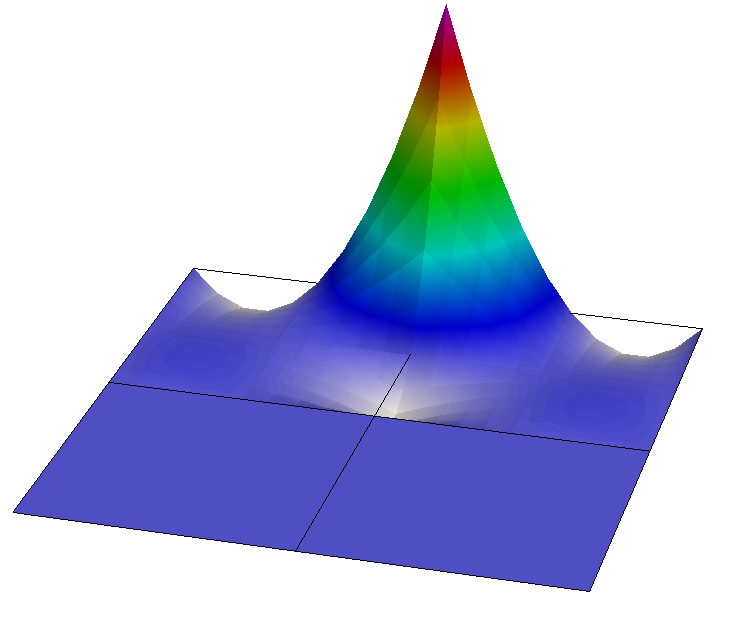
\includegraphics[height=.27\textheight]{graph/cgbasis1-16}

    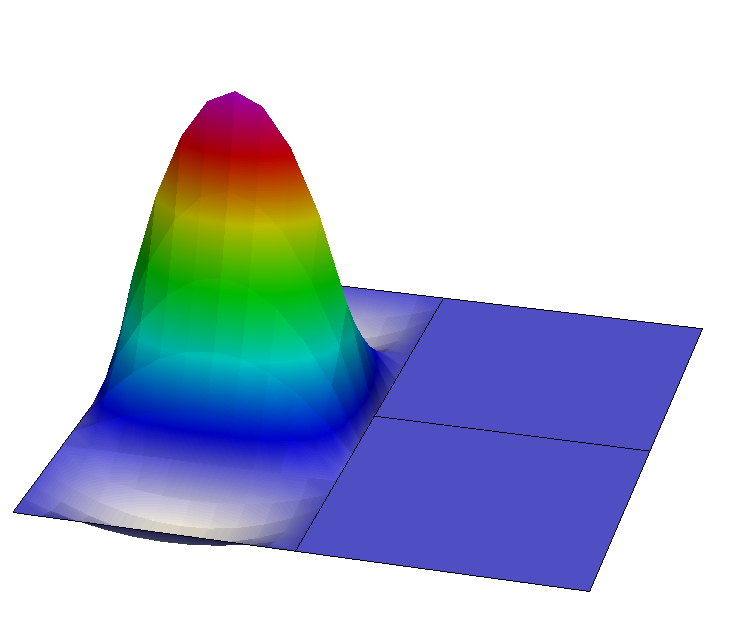
\includegraphics[height=.27\textheight]{graph/cgbasis1-07}
    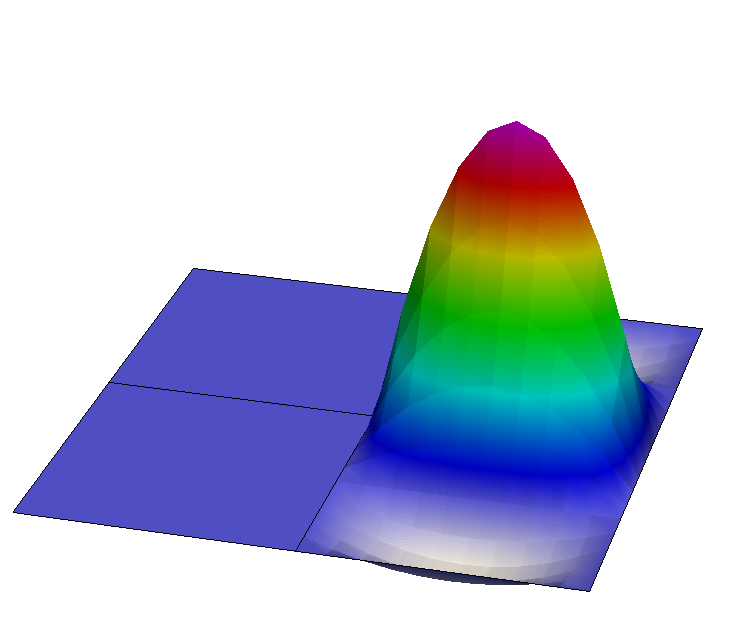
\includegraphics[height=.27\textheight]{graph/cgbasis1-13}
    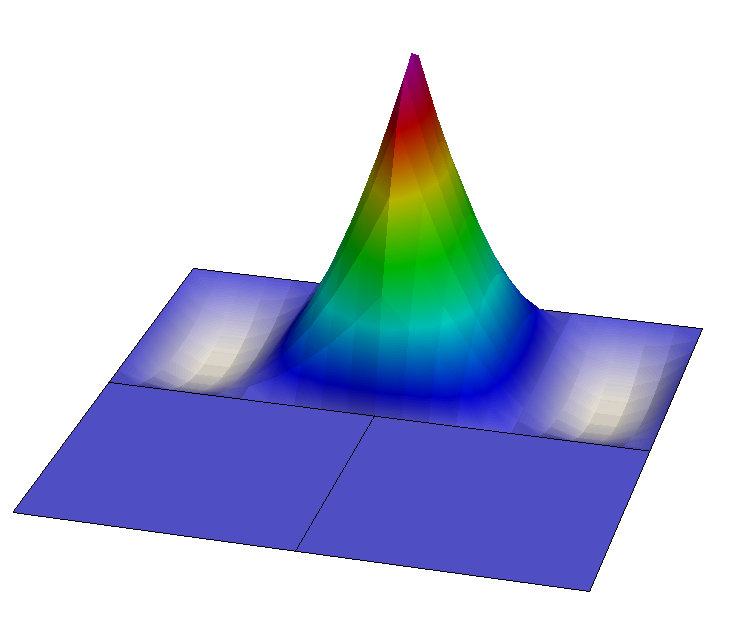
\includegraphics[height=.27\textheight]{graph/cgbasis1-18}
    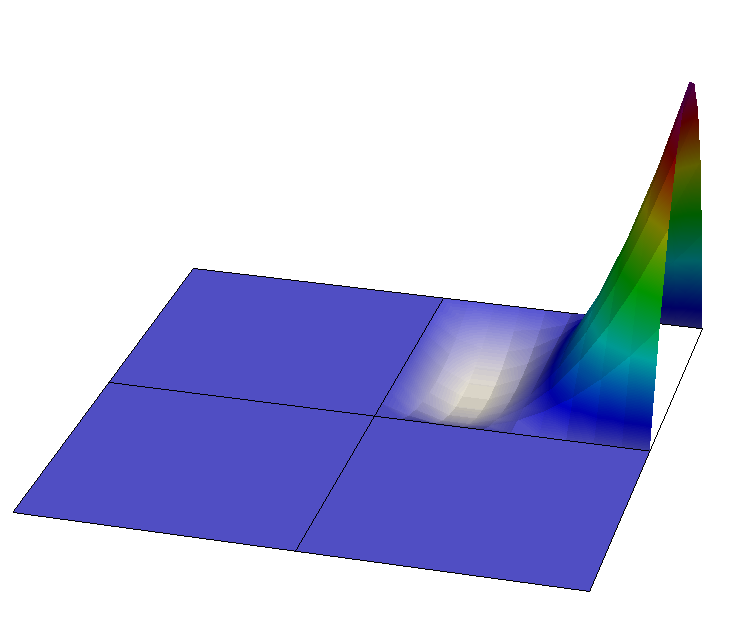
\includegraphics[height=.27\textheight]{graph/cgbasis1-22}

    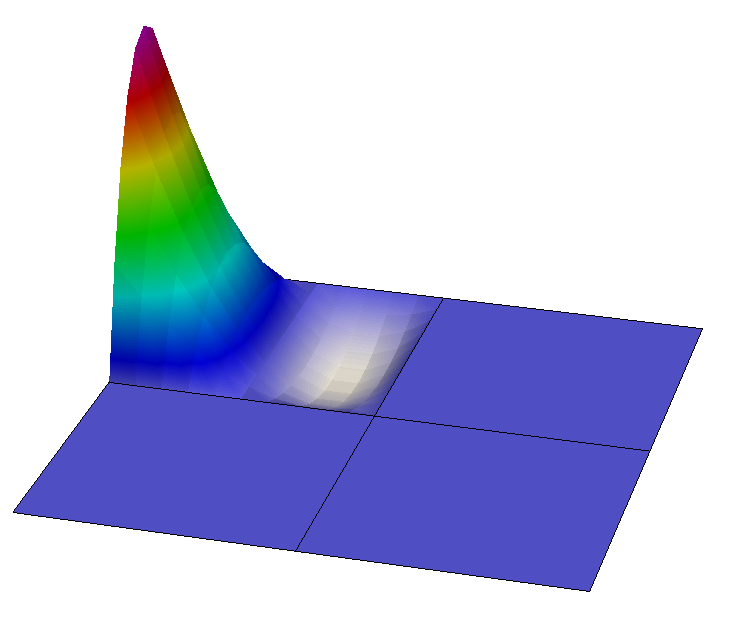
\includegraphics[height=.27\textheight]{graph/cgbasis1-17}
    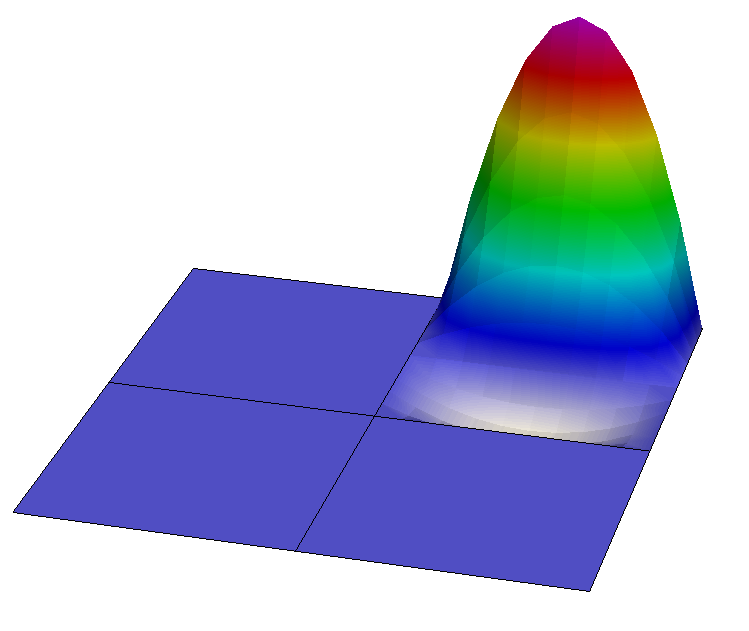
\includegraphics[height=.27\textheight]{graph/cgbasis1-23}
    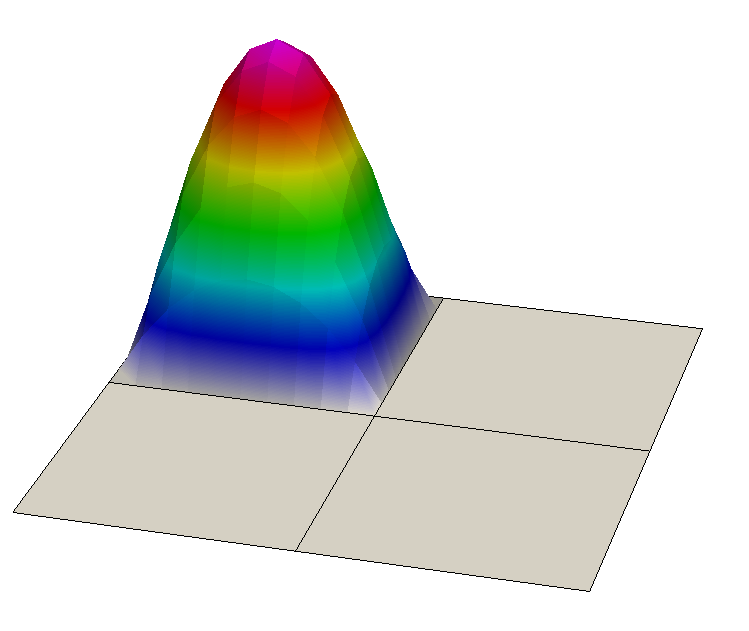
\includegraphics[height=.27\textheight]{graph/cgbasis1-20}
    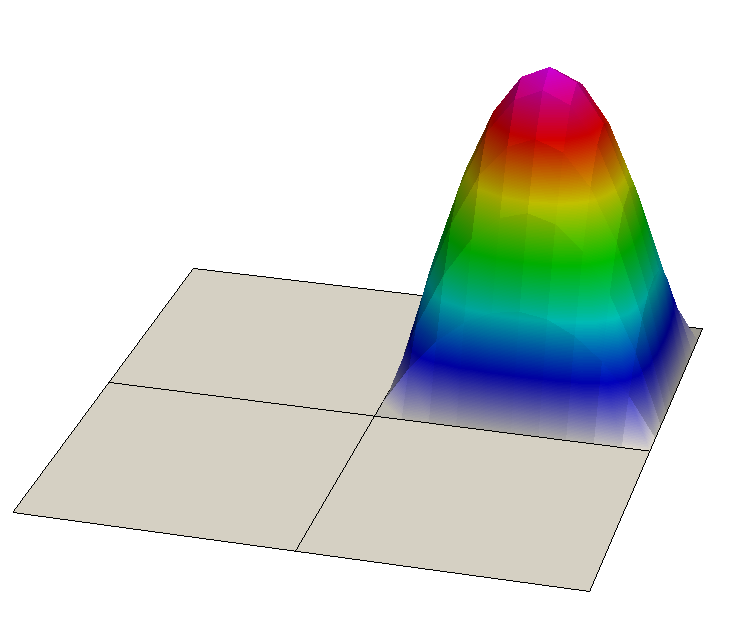
\includegraphics[height=.27\textheight]{graph/cgbasis1-24}
  \end{center}
\end{frame}

\begin{frame}
  \frametitle{Example: $Q_2$ discontinuous basis (selection)}
  \begin{center}
    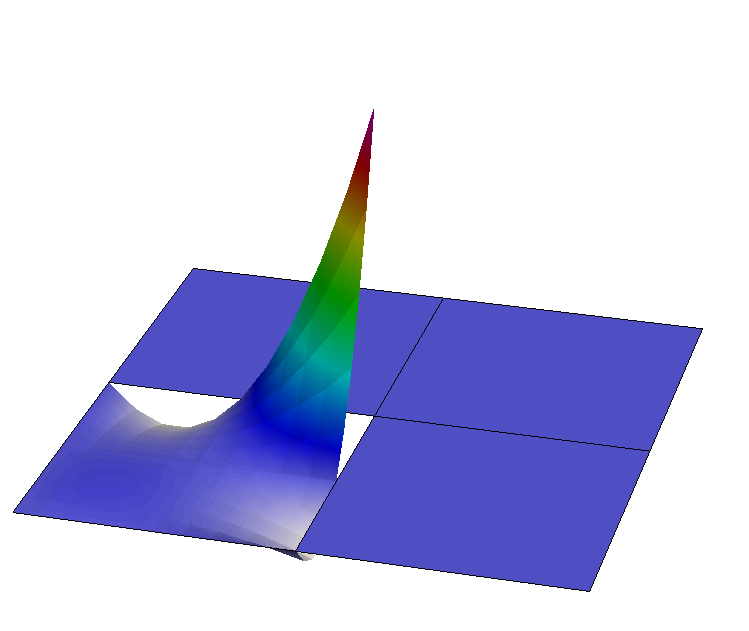
\includegraphics[height=.27\textheight]{graph/dgbasis1-08}
    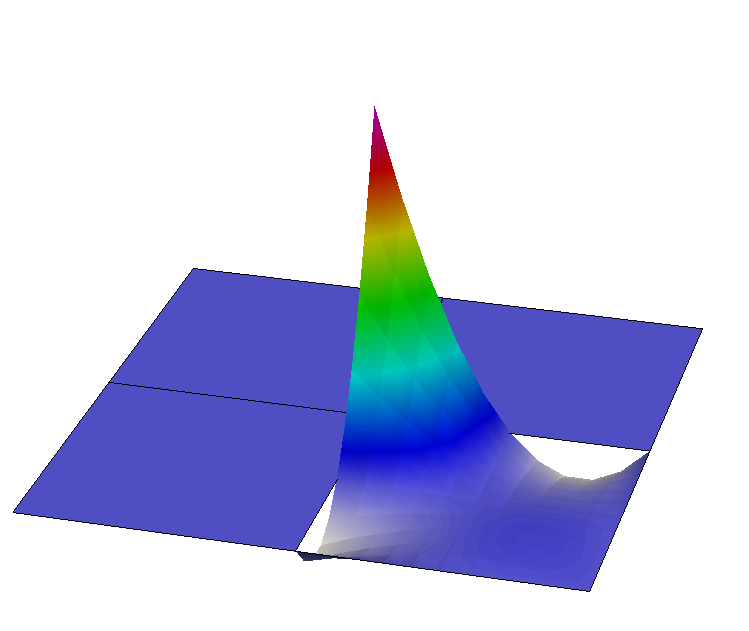
\includegraphics[height=.27\textheight]{graph/dgbasis1-15}
    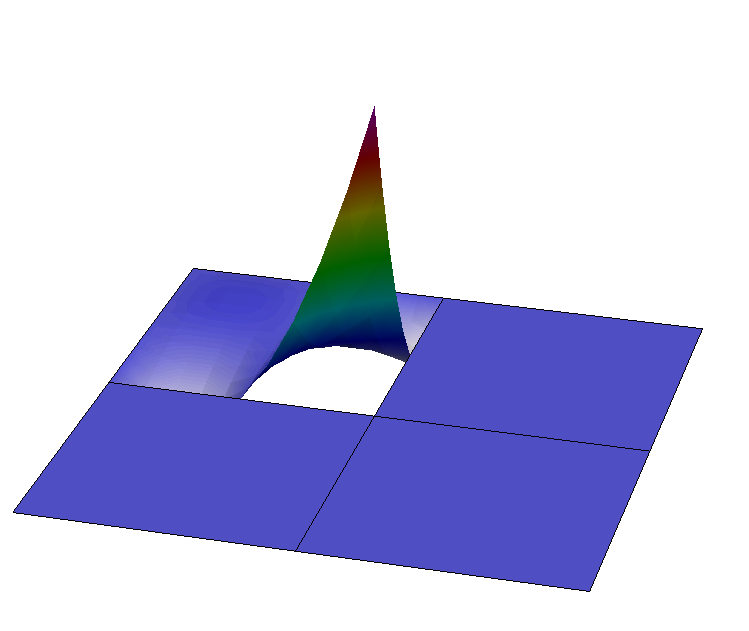
\includegraphics[height=.27\textheight]{graph/dgbasis1-20}
    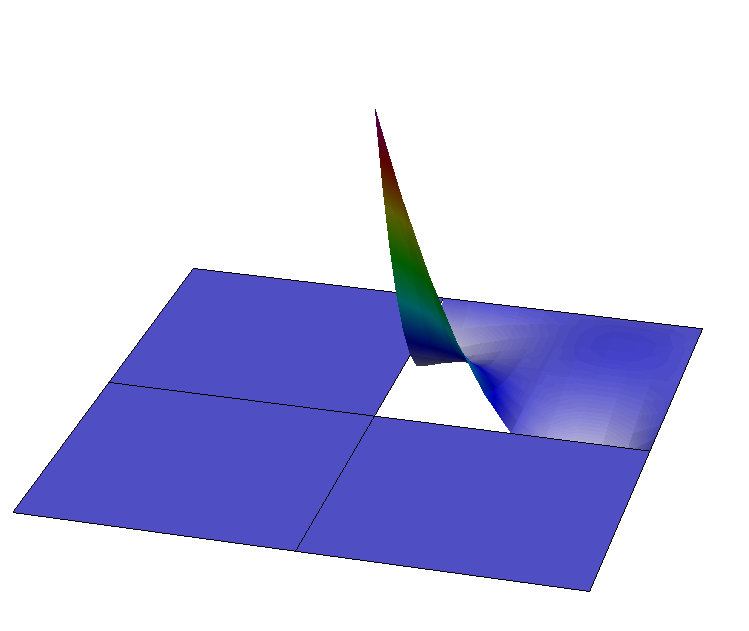
\includegraphics[height=.27\textheight]{graph/dgbasis1-27}

    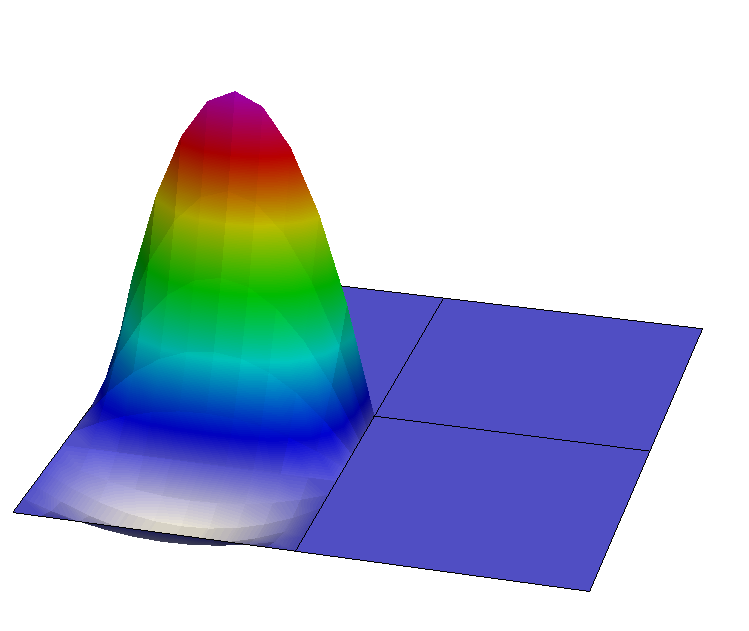
\includegraphics[height=.27\textheight]{graph/dgbasis1-07}
    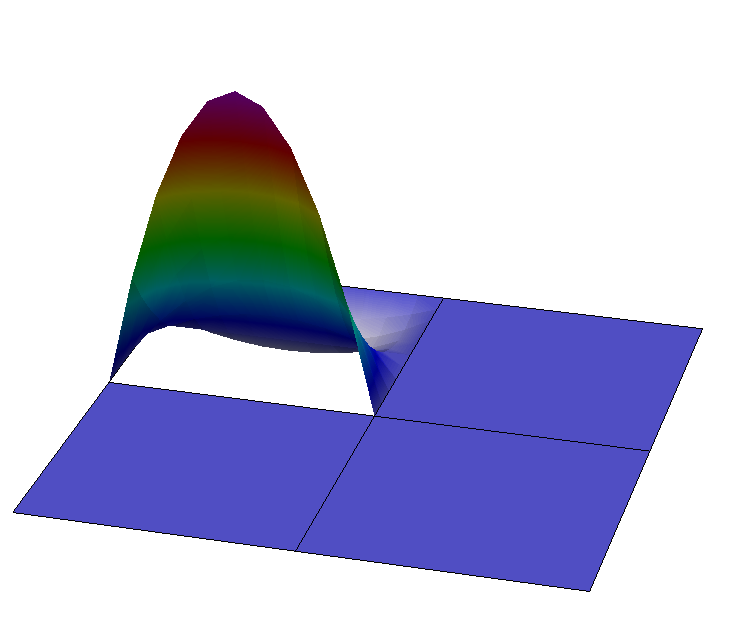
\includegraphics[height=.27\textheight]{graph/dgbasis1-19}
    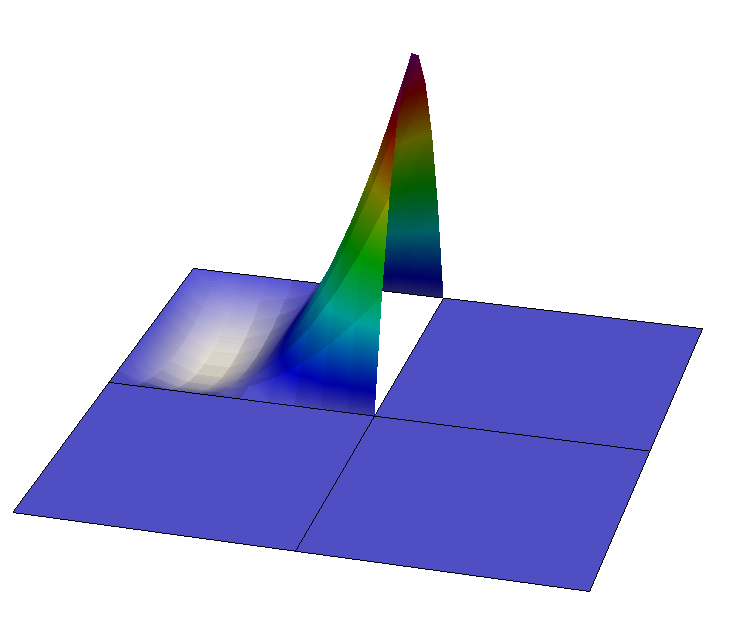
\includegraphics[height=.27\textheight]{graph/dgbasis1-23}
    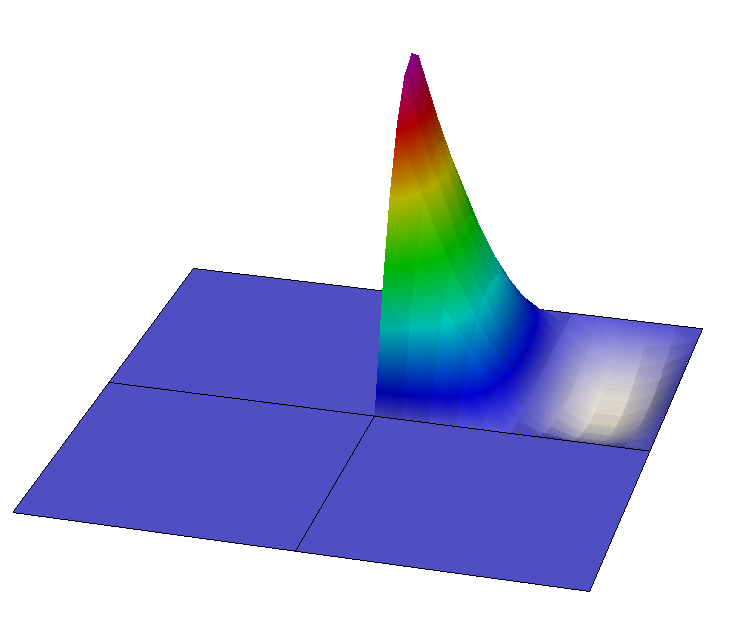
\includegraphics[height=.27\textheight]{graph/dgbasis1-30}

    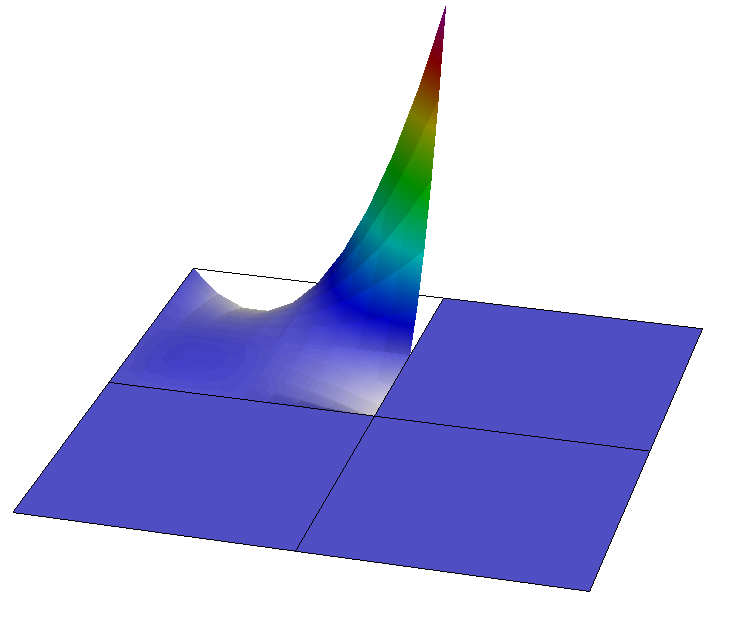
\includegraphics[height=.27\textheight]{graph/dgbasis1-26}
    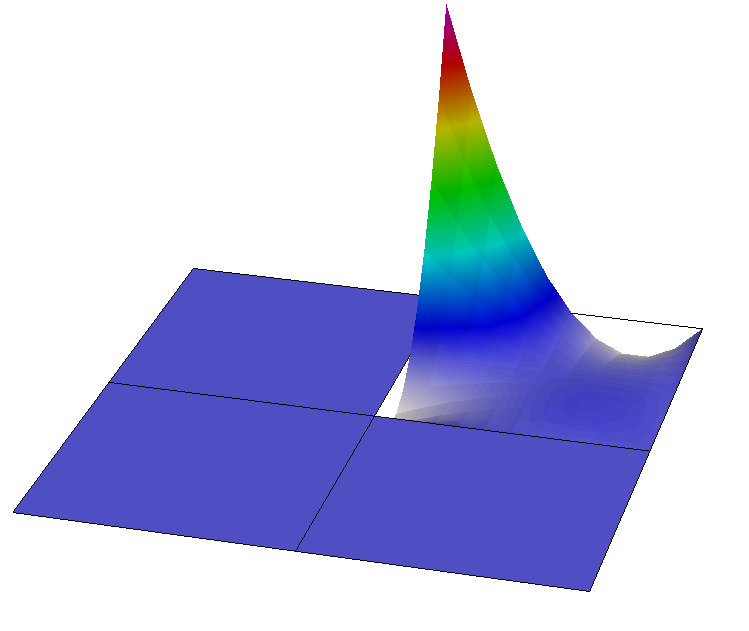
\includegraphics[height=.27\textheight]{graph/dgbasis1-33}
    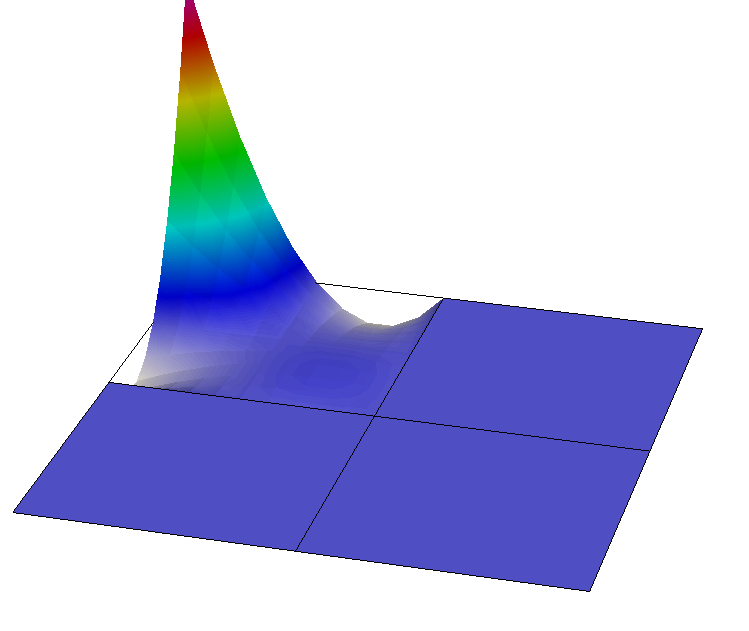
\includegraphics[height=.27\textheight]{graph/dgbasis1-24}
    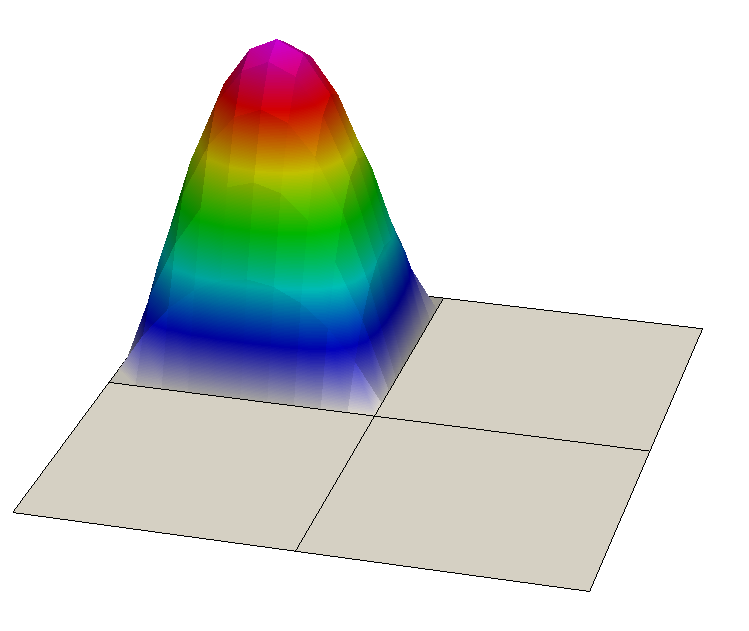
\includegraphics[height=.27\textheight]{graph/dgbasis1-22}
  \end{center}
\end{frame}

\subsubsection{Mapped finite elements}

\frame {\input{blocks/Definition-mapped-mesh.tex}}
\frame {\input{blocks/Example-mapping-linear.tex}}
\frame {\input{blocks/Example-mapping-bilinear.tex}}
\frame {\input{blocks/Definition-mapped-fe.tex}}
\frame {\input{blocks/Lemma-mapped-norms-affine.tex}}
\frame {\input{blocks/Lemma-shape-regular-transformation.tex}}
\frame {\input{blocks/Assumption-mapping-decomposition.tex}}
\frame {\input{blocks/Lemma-scaling-1.tex}}

\subsection{A priori error analysis}
\frame{\subtoc}

\frame {\input{blocks/Lemma-poincare.tex}}
\frame {\input{blocks/Lemma-bramble-hilbert.tex}}
\frame {\input{blocks/Lemma-b-h-projector.tex}}
\frame {\input{blocks/Definition-mesh-family.tex}}
\frame {\input{blocks/Definition-nodal-interpolation.tex}
  \input{blocks/Lemma-nodal-interpolation.tex}}
\frame {\input{blocks/Definition-broken-sobolev-norm.tex}}
\frame {\input{blocks/Theorem-fe-interpolation.tex}
  \input{blocks/Corollary-fe-approximation.tex}}
\frame {\input{blocks/Theorem-fe-convergence.tex}}

\subsubsection{Estimates of stronger norms}

\frame {\input{blocks/Definition-stronger-norm.tex}}
\frame {\input{blocks/Lemma-inverse-estimate.tex}}
\frame {\input{blocks/Theorem-h2-error.tex}}

\subsubsection{Estimates of weaker norms}

\frame {\input{blocks/Definition-dual-problem.tex}}
\frame {\input{blocks/Lemma-poisson-dual.tex}}
\frame {\input{blocks/Assumption-elliptic-regularity.tex}}
\frame {\input{blocks/Theorem-fe-l2.tex}
  \input {blocks/Corollary-fe-functional.tex}}

\subsubsection{Green's function and maximum norm estimates}

\frame {\input {blocks/Definition-greens-function.tex}
  \input {blocks/Theorem-greens-function-rd.tex}}
\frame {\input {blocks/Lemma-greens-function-domain.tex}}
\frame {\input {blocks/Theorem-greens-function-representation.tex}}
\frame {\input {blocks/Theorem-linfty-error.tex}}

\subsection{A posteriori error analysis}
\frame{\subtoc}

\frame {\input {blocks/Definition-a-posteriori.tex}}
\frame {\input {blocks/Definition-locally-quasi-uniform.tex}}
\frame {\input {blocks/Definition-fem-neighborhood.tex}}
\frame {\input {blocks/Theorem-clement.tex}}
\frame {\input {blocks/Theorem-scott-zhang.tex}}
\frame {\input {blocks/Theorem-schoeberl-interpolation.tex}}
\frame {\input {blocks/Definition-residual.tex}}
\frame {\input {blocks/Lemma-residual-hm1.tex}}
\frame {\input {blocks/Definition-mvl-jmp.tex}}
\frame {\input {blocks/Definition-residual-strong.tex}}
\frame {\input {blocks/Theorem-residual-upper-bound.tex}}
\frame {\input {blocks/Definition-osc.tex}}
\frame {\input {blocks/Definition-residual-estimator.tex}}
\frame {\input {blocks/Theorem-residual-estimate.tex}}

\section{Variational Crimes}
\frame{\sectoc}
\subsection{Numerical quadrature}
\frame {\input {blocks/Lemma-strang-1.tex}}
\frame {\input {blocks/Definition-tensor-product-quadrature.tex}
  \input {blocks/Lemma-tensor-product-gauss.tex}}
\frame {\input {blocks/Assumption-bilinear-form-quadrature.tex}}
\frame {\input {blocks/Definition-bilinear-quadrature.tex}}
\frame {\input {blocks/Lemma-quadrature-stability.tex}}
\frame {\input {blocks/Theorem-quadrature-error-bilinear.tex}}
\frame {\input {blocks/Lemma-product-sobolev-norm.tex}}
\frame {\input {blocks/Theorem-quadrature-error-rhs.tex}}

\section{Solving the Discrete Problem}
\frame{\sectoc}
\subsection{Richardson's method}
\frame {\input {blocks/Definition-spd-condition-number.tex}}
\frame {\input {blocks/Definition-matrix-condition-number.tex}}
\frame {\input {blocks/Lemma-richardson-error-step.tex}}
\frame {\input {blocks/Theorem-richardson-convergence1.tex}}
\frame {\input {blocks/Definition-richardson-method.tex}}
\frame {\input {blocks/Theorem-richardson-convergence2.tex}}
\frame {\input {blocks/Definition-riesz-isomorphism.tex}}
\frame {\input {blocks/Definition-p-richardson-method.tex}}
\subsection{The conjugate gradient method}
\frame{\subtoc}
\frame {\input {blocks/Definition-steepest-descent.tex}}
\frame {\input {blocks/Lemma-steepest-descent.tex}}
\frame {\input {blocks/Definition-cg-method.tex}}
\frame {\input {blocks/Definition-pcg-method.tex}}
\frame {\input {blocks/Definition-krylov-space.tex}}
\frame {\input {blocks/Lemma-cg-orthogonality.tex}}
\frame {\input {blocks/Lemma-cg-minimization.tex}}
\frame {\input {blocks/Theorem-cg-convergence.tex}}

\subsection{Condition numbers of finite element matrices}
\frame{\subtoc}
\frame {\input {blocks/Notation-up-to-a-constant.tex}}
\frame {\input {blocks/Definition-mass-stiffness.tex}}
\frame {\input {blocks/Lemma-condition-number-mass-matrix.tex}}
\frame {\input {blocks/Corollary-refined-condition-number.tex}}
\frame {\input {blocks/Theorem-condition-number-stiffness-matrix.tex}}

\subsection{Multigrid methods}
\frame {\input {blocks/Algorithm-mgm.tex}}

\section{Bibliography}
\frame{\bibliographystyle{alpha}
\bibliography{all}}
\end{document}

%%% Local Variables:
%%% mode: latex
%%% TeX-master: t
%%% End:
